\section{Samples}\label{sec:ggtt_samples}

This analysis uses data collected by the CMS experiment in pp collisions with $\sqrtS=13$\TeV during 2016, 2017 and 2018, corresponding to integrated luminosities of 36.3, 41.5 and 59.8\fbinv for each year respectively, and a total of 138\fbinv~\cite{CMS:2021xjt,CMS-PAS-LUM-17-004,CMS-PAS-LUM-18-002}. In 2018, the HLT path used for the low-mass \XYggHtt search was not introduced until after the first 5.1\fbinv of data was collected, and therefore the luminosity for this search in 2018 is reduced to 54.7\fbinv, corresponding to a total of 132\fbinv across 2016, 2017, and 2018.

Monte-Carlo (MC) simulation is generated for the signal processes at LO accuracy using \MGvATNLO v2.6.5~\cite{MadGraph}. The values of \mX (and \mY for \XYH searches) that samples are generated at is shown in \cref{fig:ggtt_sample_granularity}. In this Chapter, these values are referred to as \textit{nominal} mass points. Results are reported at these values, as well as at \textit{intermediate} mass points, which are defined in \cref{sec:search_granularity}.

\begin{figure}
  \centering
  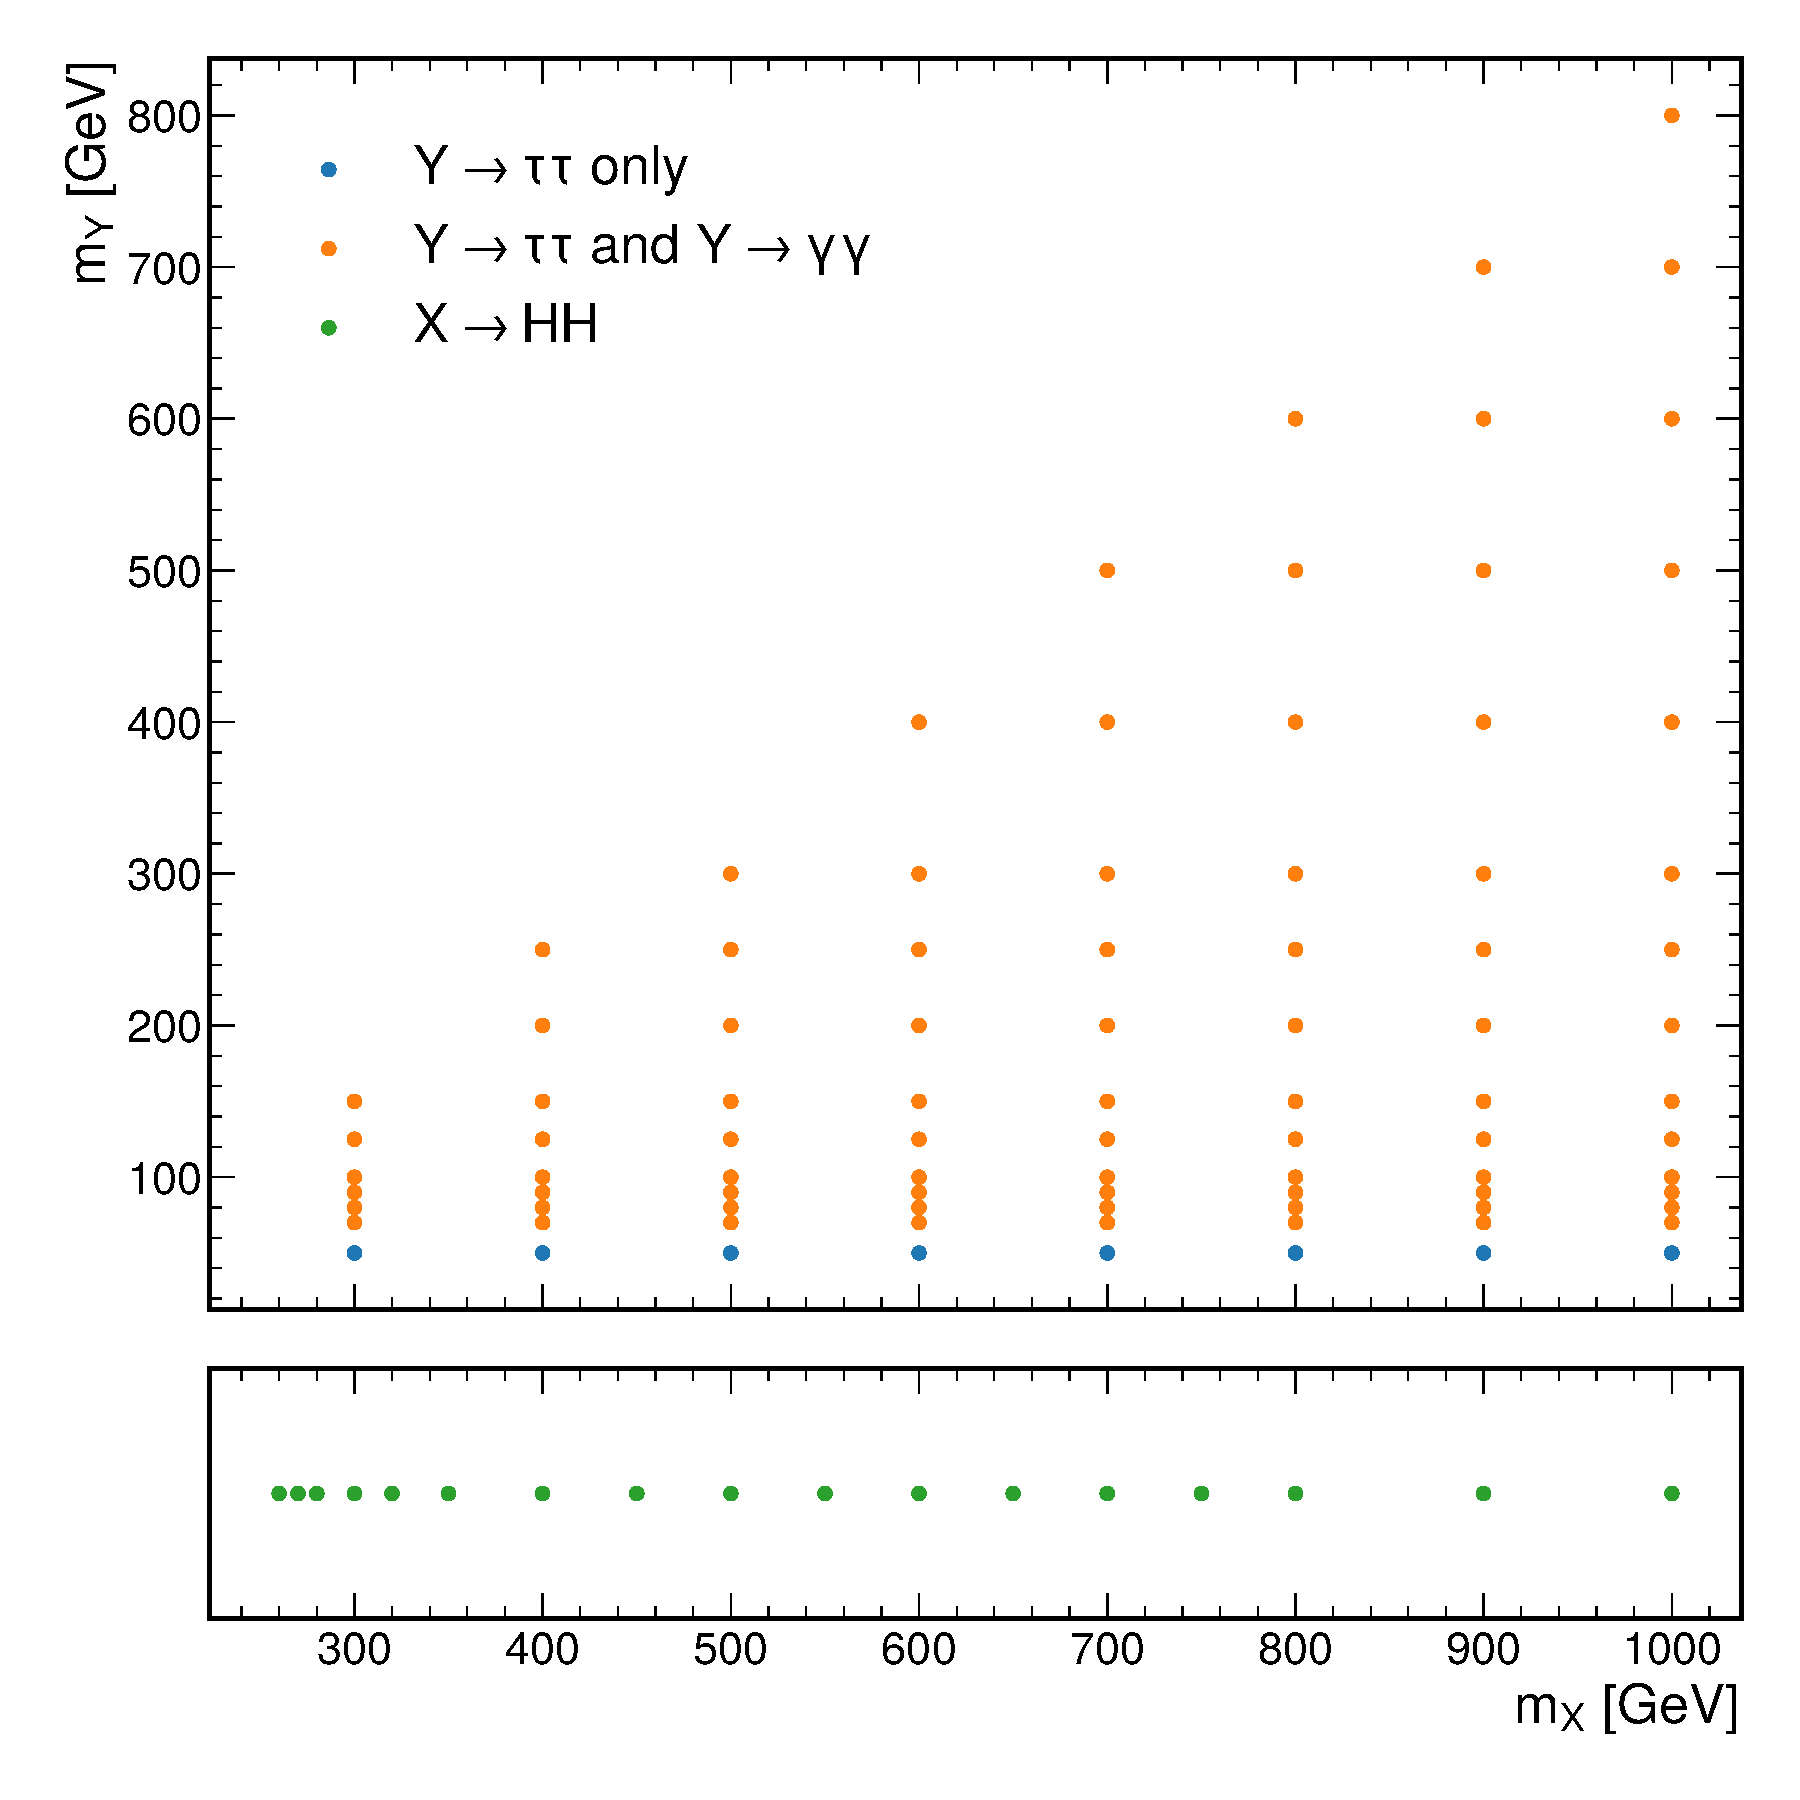
\includegraphics[width=\textwidth]{Figures/Dihiggs/NMSSM_grid.pdf}
  \caption[Nominal Mass Point Granularity]{Granularity in \mX (and \mY) that MC samples are generated at for the $\XHH$ (green), \XYggHtt (orange) and \XYttHgg (orange and blue) processes. These points define the so-called nominal mass points.}\label{fig:ggtt_sample_granularity}
\end{figure}

The \gjet and \ggjet backgrounds are modelled with \MGvATNLO v2.6.5~\cite{MadGraph,MadGraphMLM} and \SHERPA v2.2.1~\cite{10.21468/SciPostPhys.7.3.034} respectively, both at LO accuracy. The other nonresonant backgrounds: \vgamma, \ttbar, \ttgamma, and \ttgammagamma, are modelled at NLO accuracy in perturbative QCD with \MGvATNLO v2.6.5~\cite{MadGraph,MadGraphMLM,MadGraphFXFX} except for \ttbar which uses \MGvATNLO v2.6.1.

To model the SM single Higgs background, simulated events are generated for the \ggH, \VBF, \VH and \ttH production modes using \MGvATNLO v2.4.2~\cite{MadGraph,MadGraphMLM,MadGraphFXFX} at NLO accuracy in perturbative QCD. Further production modes are not simulated because their contributions are negligible. The samples are normalized to the SM cross sections and branching fractions provided by the LHC Higgs Cross Section Working Group (\cref{tab:higgs_xs,tab:higgs_brs}), which are calculated at higher orders in perturbative QCD and EW theory~\cite{LHCHiggsCrossSectionWorkingGroup:2016ypw}.

In the generation of all simulated samples, parton distribution functions are taken from the NNLO NNPDF 3.1 set~\cite{NNPDF31}. Samples are interfaced with \PYTHIA 8.240~\cite{Sjostrand:2014zea} with the CP5 tune~\cite{CMS:2015wcf,CMS:2019csb} for parton showering, fragmentation with the standard \pt-ordered parton shower scheme, and the underlying event description. Finally, the detector response is modelled using the \GEANTfour package~\cite{Agostinelli:2002hh} and the events are reconstructed using the same algorithms as for the data.

